% (find-LATEX "2022-2-C3-P1.tex")
% (defun c () (interactive) (find-LATEXsh "lualatex -record 2022-2-C3-P1.tex" :end))
% (defun C () (interactive) (find-LATEXsh "lualatex 2022-2-C3-P1.tex" "Success!!!"))
% (defun D () (interactive) (find-pdf-page      "~/LATEX/2022-2-C3-P1.pdf"))
% (defun d () (interactive) (find-pdftools-page "~/LATEX/2022-2-C3-P1.pdf"))
% (defun e () (interactive) (find-LATEX "2022-2-C3-P1.tex"))
% (defun o () (interactive) (find-LATEX "2022-1-C3-P1.tex"))
% (defun u () (interactive) (find-latex-upload-links "2022-2-C3-P1"))
% (defun v () (interactive) (find-2a '(e) '(d)))
% (defun d0 () (interactive) (find-ebuffer "2022-2-C3-P1.pdf"))
% (defun cv () (interactive) (C) (ee-kill-this-buffer) (v) (g))
% (defun oe () (interactive) (find-2a '(o) '(e)))
%          (code-eec-LATEX "2022-2-C3-P1")
% (find-pdf-page   "~/LATEX/2022-2-C3-P1.pdf")
% (find-sh0 "cp -v  ~/LATEX/2022-2-C3-P1.pdf /tmp/")
% (find-sh0 "cp -v  ~/LATEX/2022-2-C3-P1.pdf /tmp/pen/")
%     (find-xournalpp "/tmp/2022-2-C3-P1.pdf")
%   file:///home/edrx/LATEX/2022-2-C3-P1.pdf
%               file:///tmp/2022-2-C3-P1.pdf
%           file:///tmp/pen/2022-2-C3-P1.pdf
% http://angg.twu.net/LATEX/2022-2-C3-P1.pdf
% (find-LATEX "2019.mk")
% (find-sh0 "cd ~/LUA/; cp -v tikz1.lua Cabos2.lua ~/LATEX/")
% (find-CN-aula-links "2022-2-C3-P1" "3" "c3m222p1" "c3p1")

% «.defs»		(to "defs")
% «.defs-T-and-B»	(to "defs-T-and-B")
% «.title»		(to "title")
% «.links»		(to "links")
% «.barranco-defs»	(to "barranco-defs")
% «.questao-1-grids»	(to "questao-1-grids")
% «.questao-1»		(to "questao-1")
% «.questao-2»		(to "questao-2")
% «.questao-1-gab»	(to "questao-1-gab")
% «.questao-2-gab»	(to "questao-2-gab")



% <videos>
% Video (not yet):
% (find-ssr-links     "c3m222p1" "2022-2-C3-P1")
% (code-eevvideo      "c3m222p1" "2022-2-C3-P1")
% (code-eevlinksvideo "c3m222p1" "2022-2-C3-P1")
% (find-c3m222p1video "0:00")

\documentclass[oneside,12pt]{article}
\usepackage[colorlinks,citecolor=DarkRed,urlcolor=DarkRed]{hyperref} % (find-es "tex" "hyperref")
\usepackage{amsmath}
\usepackage{amsfonts}
\usepackage{amssymb}
\usepackage{pict2e}
\usepackage[x11names,svgnames]{xcolor} % (find-es "tex" "xcolor")
\usepackage{colorweb}                  % (find-es "tex" "colorweb")
\usepackage{tikz}
%
% (find-dn6 "preamble6.lua" "preamble0")
%\usepackage{proof}   % For derivation trees ("%:" lines)
%\input diagxy        % For 2D diagrams ("%D" lines)
%\xyoption{curve}     % For the ".curve=" feature in 2D diagrams
%
\usepackage{edrx21}               % (find-LATEX "edrx21.sty")
\input edrxaccents.tex            % (find-LATEX "edrxaccents.tex")
\input edrx21chars.tex            % (find-LATEX "edrx21chars.tex")
\input edrxheadfoot.tex           % (find-LATEX "edrxheadfoot.tex")
\input edrxgac2.tex               % (find-LATEX "edrxgac2.tex")
%
% (find-es "tex" "geometry")
\usepackage[a6paper, landscape,
            top=1.5cm, bottom=.25cm, left=1cm, right=1cm, includefoot
           ]{geometry}
%
\begin{document}

\catcode`\^^J=10
\directlua{dofile "dednat6load.lua"}  % (find-LATEX "dednat6load.lua")
%L dofile "Piecewise1.lua"           -- (find-LATEX "Piecewise1.lua")
%L dofile "QVis1.lua"                -- (find-LATEX "QVis1.lua")
%L dofile "Pict3D1.lua"              -- (find-LATEX "Pict3D1.lua")
%L dofile "C2Formulas1.lua"          -- (find-LATEX "C2Formulas1.lua")
%L Pict2e.__index.suffix = "%"
\pu
\def\pictgridstyle{\color{GrayPale}\linethickness{0.3pt}}
\def\pictaxesstyle{\linethickness{0.5pt}}
\def\pictnaxesstyle{\color{GrayPale}\linethickness{0.5pt}}
\celllower=2.5pt

% «defs»  (to ".defs")
% (find-LATEX "edrx21defs.tex" "colors")
% (find-LATEX "edrx21.sty")

\def\u#1{\par{\footnotesize \url{#1}}}

\def\drafturl{http://angg.twu.net/LATEX/2022-2-C3.pdf}
\def\drafturl{http://angg.twu.net/2022.2-C3.html}
\def\draftfooter{\tiny \href{\drafturl}{\jobname{}} \ColorBrown{\shorttoday{} \hours}}

% «defs-T-and-B»  (to ".defs-T-and-B")
% (c3m202p1p 6 "questao-2")
% (c3m202p1a   "questao-2")
\long\def\ColorOrange#1{{\color{orange!90!black}#1}}
\def\T(Total: #1 pts){{\bf(Total: #1)}}
\def\T(Total: #1 pts){{\bf(Total: #1 pts)}}
\def\T(Total: #1 pts){\ColorRed{\bf(Total: #1 pts)}}
\def\B       (#1 pts){\ColorOrange{\bf(#1 pts)}}




%  _____ _ _   _                               
% |_   _(_) |_| | ___   _ __   __ _  __ _  ___ 
%   | | | | __| |/ _ \ | '_ \ / _` |/ _` |/ _ \
%   | | | | |_| |  __/ | |_) | (_| | (_| |  __/
%   |_| |_|\__|_|\___| | .__/ \__,_|\__, |\___|
%                      |_|          |___/      
%
% «title»  (to ".title")
% (c3m222p1p 1 "title")
% (c3m222p1a   "title")

\thispagestyle{empty}

\begin{center}

\vspace*{1.2cm}

{\bf \Large Cálculo 3 - 2022.2}

\bsk

P1 (Primeira prova)

\bsk

Eduardo Ochs - RCN/PURO/UFF

\url{http://angg.twu.net/2022.2-C3.html}

\end{center}

\newpage

% «links»  (to ".links")
% (c3m222p1p 99 "links")
% (c3m222p1a    "links")
% (c3m222dicasp1p 2 "links")
% (c3m222dicasp1a   "links")

% «barranco-defs»  (to ".barranco-defs")

%  (eepitch-lua51)
%  (eepitch-kill)
%  (eepitch-lua51)
% -- (find-angg "LUA/lua50init.lua" "Path")
% -- (find-angg "GNUPLOT/2022-2-C3-P1.dem" "show")

%L -- Path.prepend("path", "~/LUA/?.lua")
%L require "tikz1"    -- (find-angg "LUA/tikz1.lua")
%L require "Cabos2"   -- (find-angg "LUA/Cabos2.lua" "StrGrid-tests")
%L -- (find-angg "LUA/tikz1.lua" "texbody")
%L tikzpicture = tikz [=[
%L   \begin{tikzpicture}<<options>>
%L     <<tikzbody>>
%L   \end{tikzpicture}
%L ]=]
%L sa0 = function (name, body) return format("\\sa{%s}{%s}", name, body) end
%L sa  = function (name, body) output(sa0(name, body)) end
%L tikzsa0 = function (name) return sa0(name, bitrim(tostring(tikzpicture))) end
%L tikzsa  = function (name) output(tikzsa0(name)) end
%L 
%L sg_numbers = StrGrid.from [[
%L   6 6 6 6 6 6 6 6 6 6
%L   6 6 6 6 6 6 6 6 6 6
%L   6 6 6 6 6 6 6 6 6 6
%L   5 5 5 5 4 4 4 4 4 4
%L   4 4 4 4 3 2 2 2 2 2
%L   3 3 3 3 2 1 0 0 0 0
%L   2 2 2 2 1 0 0 0 0 0
%L   1 1 1 1 0 0 0 0 0 0
%L   0 0 0 0 0 0 0 0 0 0
%L   0 0 0 0 0 0 0 0 0 0
%L   0 0 0 0 0 0 0 0 0 0
%L ]]
%L sg_reta = StrGrid.from [[
%L   .  10 .  .  .  .  .  .  .  .
%L   .  .  8  .  .  .  .  .  .  .
%L   .  .  .  6  .  .  .  .  .  .
%L   .  .  .  .  4  .  .  .  .  .
%L   .  .  .  .  .  2  .  .  .  .
%L   .  .  .  .  .  .  0  .  .  .
%L   .  .  .  .  .  .  .  -2 .  .
%L   .  .  .  .  .  .  .  . -4  .
%L   .  .  .  .  .  .  .  .  .  -6
%L   .  .  .  .  .  .  .  .  .  .
%L   .  .  .  .  .  .  .  .  .  .
%L ]]
%L sg_letters = StrGrid.from [[
%L   N N N N N N N N N N
%L   N N N N N N N N N N
%L   x x x x x x x x x x
%L   W W W x x E E E E E
%L   W W W x C x E E E E
%L   W W W x C C x x x x
%L   W W W x C x S S S S
%L   W W W x x S S S S S
%L   x x x x S S S S S S
%L   S S S S S S S S S S
%L   S S S S S S S S S S
%L ]]
%L sa("barranco: numeros", sg_numbers:drawnodes())
%L sa("barranco: reta ns", sg_reta   :drawnodes())
%L sa("barranco: letras",  sg_letters:drawletters())
%L tikzbody = tikz [=[
%L   [scale=0.8]
%L   \draw [color=gray!30] (0,0) grid (9,10);
%L   \ga{barranco: numeros}
%L   \ga{barranco: letras}
%L   <<orangelines>>
%L ]=]
%L tikzsa("barranco")
%L orangelines = [=[
%L   \draw [color=orange, very thick]
%L      (0,8) -- (9,8)
%L      (3,2) -- (3,8) -- (6,5)
%L      (0,2) -- (3,2) -- (6,5) -- (9,5);
%L   \draw [color=red, very thick] (0,4) -- ++(6,6);
%L   \draw [color=red, very thick] (0,2) -- ++(8,8);
%L   \draw [color=red, very thick] (0,0) -- ++(9,9);
%L ]=]
%L tikzsa("barranco com linhas")
\pu


%%L tikzbody = tikz [=[
%%L   [scale=0.8]
%%L   \draw [color=gray!30] (0,0) grid (9,10);
%%L   \ga{barranco: numeros}
%%L   \ga{barranco: letras}
%%L   <<orangelines>>
%%L ]=]


\sa{barranco: orange lines}{
  \draw [color=orange, very thick]
     (0,8) -- (9,8)
     (3,2) -- (3,8) -- (6,5)
     (0,2) -- (3,2) -- (6,5) -- (9,5);
  }
\sa{barranco: red lines}{
  \draw [color=red, very thick] (0,4) -- ++(6,6);
  }

\def\drawx (#1,#2);{\node at (#1,#2) {$×$};}
\def\drawN (#1,#2);{\node at (#1,#2) {$\bullet$};}
\def\drawS (#1,#2);{\node at (#1,#2) {$\bullet$};}
\def\drawW (#1,#2);{\draw [->] (#1,#2) -- ++ (0,0.33);}
\def\drawC (#1,#2);{\draw [->] (#1,#2) -- ++ (-0.33,0.33);}
\def\drawE (#1,#2);{\draw [->] (#1,#2) -- ++ (0,0.66);}

\sa{barranco: grid}{
  \draw [color=gray!30] (0,0) grid (9,10);
  }

\sa{barranco}{\begin{tikzpicture}%
    [scale=0.8]
    \ga{barranco: grid}
    \ga{barranco: numeros}
  \end{tikzpicture}}

\sa{barranco gab item a}{\begin{tikzpicture}%
    [scale=0.8]
    \ga{barranco: grid}
    \ga{barranco: numeros}
    \ga{barranco: orange lines}
  \end{tikzpicture}}

\sa{barranco gab item c}{\begin{tikzpicture}%
    [scale=0.8]
    \ga{barranco: grid}
    \ga{barranco: reta ns}
    \ga{barranco: orange lines}
  \end{tikzpicture}}

\sa{barranco gab item e}{\begin{tikzpicture}%
    [scale=0.8]
    \ga{barranco: grid}
    \ga{barranco: orange lines}
    \ga{barranco: letras}
  \end{tikzpicture}}

\sa{barranco gab item f}{\begin{tikzpicture}%
    [scale=0.8]
    \ga{barranco: grid}
    \ga{barranco: numeros}
    \ga{barranco: orange lines}
    \ga{barranco: red lines}
  \end{tikzpicture}}

\sa{barranco gab item f parte 2}{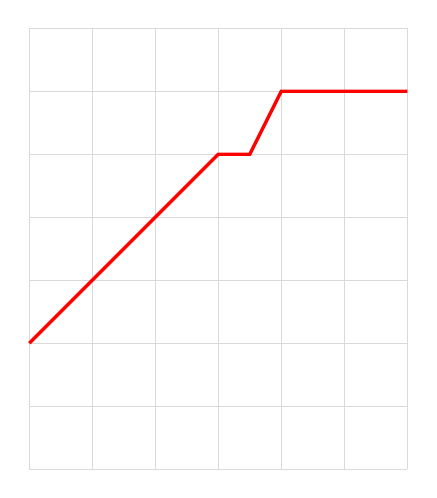
\begin{tikzpicture}%
    [scale=0.8]
    \draw [color=gray!30] (0,0) grid (6,7);
    \draw [color=red, very thick] (0,2) -- (3,5) -- (3.5,5) -- (4,6) -- (6,6);
  \end{tikzpicture}}


\newpage

% «questao-1-grids»  (to ".questao-1-grids")
% (c3m222p1p 2 "questao-1-grids")
% (c3m222p1a   "questao-1-grids")

\def\barra {\scalebox{0.4}{$\ga{barranco}$}}
\def\barral{\ga{barranco com linhas}}

$\begin{matrix}
 \barra & \barra & \barra \\ \\
 \barra & \barra & \barra \\
 \end{matrix}
$

% $\barral$

%$\ga{barranco}$

% Idéias:
% Na questão sobre curvas de nivel e campos gradientes
% usar primeiro uma hiperbole careta e depois uma
% hiperbole torta.

\newpage

%   ___                  _                _ 
%  / _ \ _   _  ___  ___| |_ __ _  ___   / |
% | | | | | | |/ _ \/ __| __/ _` |/ _ \  | |
% | |_| | |_| |  __/\__ \ || (_| | (_) | | |
%  \__\_\\__,_|\___||___/\__\__,_|\___/  |_|
%                                           
% «questao-1»  (to ".questao-1")
% (c3m222p1p 3 "questao-1")
% (c3m222p1a   "questao-1")

{\bf Questão 1}

\scalebox{0.6}{\def\colwidth{9cm}\firstcol{

\vspace*{-0.5cm}

\T(Total: 6.0 pts)

O diagrama de numerozinhos da folha anterior corresponde a uma
superfície $z=F(x,y)$ que tem 5 faces. Também é possível interpretá-lo
como uma superfície com 6 ou mais faces, mas vamos considerar que a
superfície com só 5 faces é que é a correta.

\msk

a) \B (1.0 pts) Mostre como dividir o plano em 5 polígonos que são as
projeções destas faces.

\msk

b) \B (1.0 pts) Chame estas faces de face N (``norte''), S (``sul''),
W (``oeste''), C (``centro''), E (``leste''), e chame as equações dos
planos delas de $F_N(x,y)$, $F_S(x,y)$, $F_W(x,y)$, $F_C(x,y)$, e
$F_E(x,y)$. Dê as equações destes planos.

\msk

c) \B (1.0 pts) Sejam:
%
$$\begin{array}{rcl}
  P_C &=& \setofxyzst{z = F_C(x,y)}, \\
  P_E &=& \setofxyzst{z = F_E(x,y)}, \\
  r &=& P_C ∩ P_E. \\
  \end{array}
$$

Represente a reta $r$ graficamente como numerozinhos.

}\anothercol{

  d) \B (0.5 pts) Dê uma parametrização para a reta do item anterior.
  Use notação de conjuntos.

  \msk

  e) \B (1.0 pts) Seja
  %
  $$A \;=\; \{0,1,\ldots,9\} × \{0,1,\ldots,10\};$$

  note que os numerozinhos do diagrama de numerozinhos estão todos
  sobre pontos de $A$. Para cada ponto $(x,y)∈A$ represente
  graficamente $(x,y)+\frac13 \vec∇F(x,y)$.

  \ssk

  Obs: quando $\vec∇F(x,y)=0$ desenhe uma bolinha preta sobre o ponto
  $(x,y)$, e quando $\vec∇F(x,y)$ não existir faça um `$×$' sobre o
  numerozinho que está no ponto $(x,y)$.

  \msk

  f) \B (1.5 pts) Sejam
  %
  $$\begin{array}{rcl}
    Q(t) &=& (0,4) + t\VEC{1,1}, \\
    (x(t),y(t)) &=& Q(t), \\
    h(t) &=& F(x(t),y(t)). \\
    \end{array}
  $$

  Faça o gráfico da função $h(t)$. Considere que o domínio dela é o
  intervalo $[0,6]$.

}}


\newpage

%   ___                  _                ____  
%  / _ \ _   _  ___  ___| |_ __ _  ___   |___ \ 
% | | | | | | |/ _ \/ __| __/ _` |/ _ \    __) |
% | |_| | |_| |  __/\__ \ || (_| | (_) |  / __/ 
%  \__\_\\__,_|\___||___/\__\__,_|\___/  |_____|
%                                               
% «questao-2»  (to ".questao-2")
% (c3m222p1p 4 "questao-2")
% (c3m222p1a   "questao-2")

{\bf Questão 2}


\scalebox{0.6}{\def\colwidth{9cm}\firstcol{

\vspace*{-0.5cm}

\T(Total: 4.5 pts)

Seja
%
$$F(x,y) = 2x^2 -xy -y^2.$$

Nesta questão você vai ter que fazer várias cópias do diagrama de
numerozinhos da função $F(x,y)$ para os pontos com
$x,y∈\{-2,-1,0,1,2\}$. Os numerozinhos vão ser estes aqui:
%
$$\begin{array}{rrrrr}
  8 &  0 &  -4 & -4 &  0 \\
  9 &  2 &  -1 &  0 &  5 \\
  8 &  2 &   0 &  2 &  8 \\
  5 &  0 &  -1 &  2 &  9 \\
  0 & -4 &  -4 &  0 &  8 \\
  \end{array}
$$

a) \B (1.0 pts) Desenhe o ``campo gradiente'' da função $F$ nestes
pontos, mas multiplicando cada $\vec∇F(x,y)$ por $\frac{1}{10}$ pros
vetores não ficarem uns em cima dos outros. Deixa eu traduzir isso pra
termos mais básicos: faça uma cópia do diagrama de numerozinhos da
$F(x,y)$, e sobre cada $(x,y)$ com $x,y∈\{-2,-1,0,1,2\}$ desenhe a
seta $(x,y)+\frac{1}{10}\vec∇F(x,y)$.

}\anothercol{

  b) \B (3.5 pts) Faça uma outra cópia desse diagrama de numerozinhos
  e desenhe sobre ela as curvas de nível da função $F(x,y)$ para
  $z=0$, $z=2$, $z=5$, $z=-1$ e $z=-2$.

  \bsk

  {\bf Dicas:}

  1) O vetor gradiente num ponto $(x,y)$ é sempre ortogonal à curva de
  nível que passa pelo ponto $(x,y)$.

  2) Faça quantos rascunhos quiser. Eu só vou corrigir seus desenhos
  pros itens (a) e (b) que disserem ``versão final'', e eles têm que
  ser os mais caprichados possíveis.


}}


\newpage

%   ___                  _                _               _     
%  / _ \ _   _  ___  ___| |_ __ _  ___   / |   __ _  __ _| |__  
% | | | | | | |/ _ \/ __| __/ _` |/ _ \  | |  / _` |/ _` | '_ \ 
% | |_| | |_| |  __/\__ \ || (_| | (_) | | | | (_| | (_| | |_) |
%  \__\_\\__,_|\___||___/\__\__,_|\___/  |_|  \__, |\__,_|_.__/ 
%                                             |___/             
% «questao-1-gab»  (to ".questao-1-gab")
% (c3m222p1p 5 "questao-1-gab")
% (c3m222p1a   "questao-1-gab")

{\bf Questão 1: gabarito}

\def\sb#1{\scalebox{0.3}{#1}}
\def\sb#1{\ensuremath{\myvcenter{$\scalebox{0.6}{#1}$}}}

\scalebox{0.48}{\def\colwidth{8cm}\firstcol{

\vspace*{0cm}

a) \sb{\ga{barranco gab item a}}

\msk

b) $\begin{array}[c]{rcl}
      F_N(x,y) &=& 6 \\
      F_W(x,y) &=& -2 + y \\
      F_C(x,y) &=& 1 - x + y \\
      F_E(x,y) &=& -10 + 2y \\
      F_S(x,y) &=& 0 \\
    \end{array}
   $

\msk

c) \sb{\ga{barranco gab item c}}

\msk

d) $\setofst{(6,5,0) + t\VEC{-1,1,2}}{t∈\R}$

}\anothercol{

\vspace*{0cm}

e) \sb{\ga{barranco gab item e}}

\msk

f) \hbox{%
     \sb{\ga{barranco gab item f}}
     $⇒$
     \sb{\ga{barranco gab item f parte 2}}
     \hss
   }

}}


\newpage

%   ___                  _                ____                _     
%  / _ \ _   _  ___  ___| |_ __ _  ___   |___ \    __ _  __ _| |__  
% | | | | | | |/ _ \/ __| __/ _` |/ _ \    __) |  / _` |/ _` | '_ \ 
% | |_| | |_| |  __/\__ \ || (_| | (_) |  / __/  | (_| | (_| | |_) |
%  \__\_\\__,_|\___||___/\__\__,_|\___/  |_____|  \__, |\__,_|_.__/ 
%                                                 |___/             
% «questao-2-gab»  (to ".questao-2-gab")
% (find-es "maxima" "2022-2-C3-P1")

% (c3m222p1p 6 "questao-2-gab")
% (c3m222p1a   "questao-2-gab")

{\bf Questão 2: gabarito}

\bsk

%L F   = function (x,y) return 2*x^2 - x*y - y^2 end
%L F_x = function (x,y) return 4*x   -   y       end
%L F_y = function (x,y) return       - x   - 2*y end
%L so_numbers = StrOut.new()
%L so_arrows  = StrOut.new()
%L for y=2,-2,-1 do
%L   for x=-2,2 do
%L     so_numbers:printf("\\node at (%d,%d) {%d};\n", x, y, F(x,y))
%L     so_arrows :pprintf("\\draw [color=red, ->] (%s,%s) -- ++ (%s,%s);\n",
%L                        x, y, F_x(x,y)/10, F_y(x,y)/10)
%L   end
%L end
%L sa("questao 2: numeros", so_numbers:tostring00())
%L sa("questao 2: setas",   so_arrows:tostring00())
\pu

% (setq eepitch-preprocess-regexp "^")
% (setq eepitch-preprocess-regexp "^%T ")
%
%T  (eepitch-maxima)
%T  (eepitch-kill)
%T  (eepitch-maxima)
%T F : 2*x^2 - x*y - y^2;
%T sols : solve(F-z, x);
%T sol1 : rhs(sols[1]);
%T sol2 : rhs(sols[2]);
%T display2d:false$
%T sol1;
%T sol2;
%T display2d:true$



\sa{level curve for z=0}{
  (-2,-2)--(2,2)
  (1,-2)--(-1,2)
}
\sa{level curve for z=-1}{
  (-0.823,2)--(-0.791,1.947)--(-0.759,1.894)--(-0.726,1.841)--(-0.693,1.789)--(-0.659,1.736)--(-0.625,1.683)--(-0.59,1.63)--(-0.554,1.577)--(-0.517,1.524)--(-0.479,1.472)--(-0.44,1.419)--(-0.4,1.366)--(-0.357,1.313)--(-0.312,1.26)--(-0.264,1.207)--(-0.211,1.154)--(-0.152,1.102)--(-0.082,1.049)--(0.008,0.996)--(0.222,0.943)--
  (0.25,0.943)--(0.489,0.996)--(0.607,1.049)--(0.703,1.102)--(0.788,1.154)--(0.867,1.207)--(0.942,1.26)--(1.014,1.313)--(1.083,1.366)--(1.15,1.419)--(1.215,1.471)--(1.279,1.524)--(1.343,1.577)--(1.405,1.63)--(1.466,1.683)--(1.527,1.736)--(1.587,1.789)--(1.647,1.841)--(1.706,1.894)--(1.765,1.947)--(1.823,2)
  (-1.823,-2)--(-1.765,-1.947)--(-1.706,-1.894)--(-1.647,-1.841)--(-1.587,-1.789)--(-1.527,-1.736)--(-1.466,-1.683)--(-1.405,-1.63)--(-1.343,-1.577)--(-1.279,-1.524)--(-1.215,-1.472)--(-1.15,-1.419)--(-1.083,-1.366)--(-1.014,-1.313)--(-0.942,-1.26)--(-0.867,-1.207)--(-0.788,-1.154)--(-0.703,-1.102)--(-0.607,-1.049)--(-0.489,-0.996)--(-0.25,-0.943)--
  (-0.222,-0.943)--(-0.008,-0.996)--(0.082,-1.049)--(0.152,-1.102)--(0.211,-1.154)--(0.264,-1.207)--(0.312,-1.26)--(0.357,-1.313)--(0.4,-1.366)--(0.44,-1.419)--(0.479,-1.471)--(0.517,-1.524)--(0.554,-1.577)--(0.59,-1.63)--(0.625,-1.683)--(0.659,-1.736)--(0.693,-1.789)--(0.726,-1.841)--(0.759,-1.894)--(0.791,-1.947)--(0.823,-2)
}
\sa{level curve for z=-2}{
  (-0.618,2)--(-0.593,1.967)--(-0.567,1.933)--(-0.54,1.9)--(-0.513,1.867)--(-0.486,1.833)--(-0.457,1.8)--(-0.428,1.767)--(-0.398,1.734)--(-0.366,1.7)--(-0.334,1.667)--(-0.3,1.634)--(-0.264,1.6)--(-0.226,1.567)--(-0.185,1.534)--(-0.141,1.501)--(-0.092,1.467)--(-0.037,1.434)--(0.029,1.401)--(0.115,1.367)--(0.302,1.334)--
  (0.365,1.334)--(0.569,1.367)--(0.672,1.401)--(0.754,1.434)--(0.826,1.467)--(0.891,1.501)--(0.952,1.534)--(1.009,1.567)--(1.064,1.6)--(1.116,1.634)--(1.167,1.667)--(1.216,1.7)--(1.264,1.734)--(1.311,1.767)--(1.357,1.8)--(1.402,1.833)--(1.447,1.867)--(1.49,1.9)--(1.533,1.933)--(1.576,1.967)--(1.618,2)
  (-1.618,-2)--(-1.576,-1.967)--(-1.533,-1.933)--(-1.49,-1.9)--(-1.447,-1.867)--(-1.402,-1.833)--(-1.357,-1.8)--(-1.311,-1.767)--(-1.264,-1.734)--(-1.216,-1.7)--(-1.167,-1.667)--(-1.116,-1.634)--(-1.064,-1.6)--(-1.009,-1.567)--(-0.952,-1.534)--(-0.891,-1.501)--(-0.826,-1.467)--(-0.754,-1.434)--(-0.672,-1.401)--(-0.569,-1.367)--(-0.365,-1.334)--
  (-0.302,-1.334)--(-0.115,-1.367)--(-0.029,-1.401)--(0.037,-1.434)--(0.092,-1.467)--(0.141,-1.501)--(0.185,-1.534)--(0.226,-1.567)--(0.264,-1.6)--(0.3,-1.634)--(0.334,-1.667)--(0.366,-1.7)--(0.398,-1.734)--(0.428,-1.767)--(0.457,-1.8)--(0.486,-1.833)--(0.513,-1.867)--(0.54,-1.9)--(0.567,-1.933)--(0.593,-1.967)--(0.618,-2)
}
\sa{level curve for z=2}{
  (-1.995,-1.64)--(-1.846,-1.458)--(-1.703,-1.276)--(-1.567,-1.094)--(-1.44,-0.912)--(-1.323,-0.73)--(-1.218,-0.548)--(-1.128,-0.366)--(-1.055,-0.184)--(-1.001,-0.002)--(-0.964,0.18)--(-0.946,0.362)--(-0.944,0.544)--(-0.957,0.726)--(-0.983,0.908)--(-1.019,1.09)--(-1.064,1.272)--(-1.116,1.454)--(-1.174,1.636)--(-1.236,1.818)--(-1.303,2)
  (1.303,-2)--(1.236,-1.818)--(1.174,-1.636)--(1.116,-1.454)--(1.064,-1.272)--(1.019,-1.09)--(0.983,-0.908)--(0.957,-0.726)--(0.944,-0.544)--(0.946,-0.362)--(0.964,-0.18)--(1.001,0.002)--(1.055,0.184)--(1.128,0.366)--(1.218,0.548)--(1.323,0.73)--(1.44,0.912)--(1.567,1.094)--(1.703,1.276)--(1.846,1.458)--(1.995,1.64)
}
\sa{level curve for z=5}{
  (-2,-1)--(-1.917,-0.85)--(-1.841,-0.7)--(-1.772,-0.55)--(-1.709,-0.4)--(-1.655,-0.25)--(-1.608,-0.1)--(-1.569,0.05)--(-1.538,0.2)--(-1.515,0.35)--(-1.5,0.5)--(-1.492,0.65)--(-1.491,0.8)--(-1.497,0.95)--(-1.508,1.1)--(-1.526,1.25)--(-1.548,1.4)--(-1.575,1.55)--(-1.606,1.7)--(-1.641,1.85)--(-1.679,2)
  (1.679,-2)--(1.641,-1.85)--(1.606,-1.7)--(1.575,-1.55)--(1.548,-1.4)--(1.526,-1.25)--(1.508,-1.1)--(1.497,-0.95)--(1.491,-0.8)--(1.492,-0.65)--(1.5,-0.5)--(1.515,-0.35)--(1.538,-0.2)--(1.569,-0.05)--(1.608,0.1)--(1.655,0.25)--(1.709,0.4)--(1.772,0.55)--(1.841,0.7)--(1.917,0.85)--(2,1)
}
\sa{level curves}{
  \ga{level curve for z=0}
  \ga{level curve for z=-1}
  \ga{level curve for z=-2}
  \ga{level curve for z=2}
  \ga{level curve for z=5}
}


\sa{questao 2a}{\begin{tikzpicture}%
    [scale=1.2]
    \draw [color=gray!20] (-2,-2) grid (2,2);
    \draw [color=orange] \ga{level curve for z=0};
    \ga{questao 2: numeros}
    \ga{questao 2: setas}
  \end{tikzpicture}}

\sa{questao 2b}{\begin{tikzpicture}%
    [scale=1.2]
    \draw [color=gray!20] (-2,-2) grid (2,2);
    \draw [color=orange] \ga{level curves};
    % \ga{questao 2: numeros}
    \ga{questao 2: setas}
  \end{tikzpicture}}

\scalebox{0.75}{
\ga{questao 2a}
\qquad
\ga{questao 2b}
}



%\printbibliography

\GenericWarning{Success:}{Success!!!}  % Used by `M-x cv'

\end{document}


% Local Variables:
% coding: utf-8-unix
% ee-tla: "c3p1"
% ee-tla: "c3m222p1"
% End:
